\documentclass{article}
\usepackage{graphicx}
\usepackage{float}
\usepackage{subcaption}

\begin{document}

\section{Last Time}

\subsection{Concentrate on the answer they choose}
\begin{figure}[H]
  \centering
  % First row of images
  \begin{subcaptionbox}{Answered A\label{fig:A_dt_g}}[0.45\textwidth]
    {\centering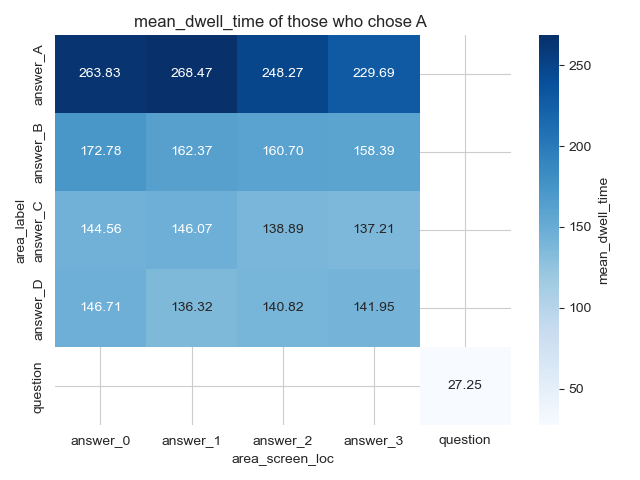
\includegraphics[width=\linewidth]{plots/matrix_plots/matrix_mean_dwell_time_A_gatherers.png}}
  \end{subcaptionbox}
  \hfill
  \begin{subcaptionbox}{Answered B\label{fig:B_dt_g}}[0.45\textwidth]
    {\centering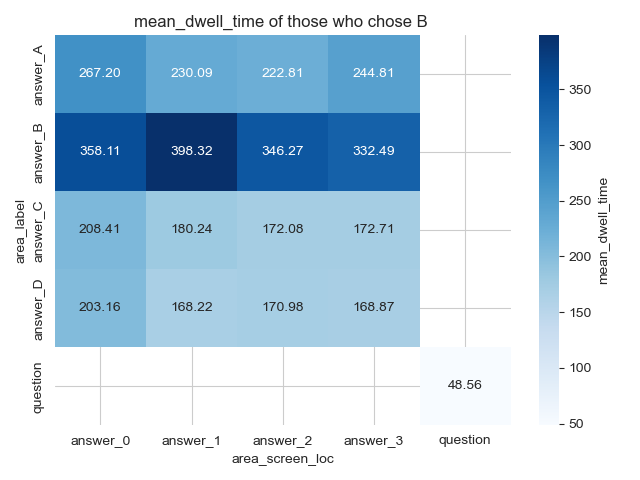
\includegraphics[width=\linewidth]{plots/matrix_plots/matrix_mean_dwell_time_B_gatherers.png}}
  \end{subcaptionbox}
    \vspace{1em} % Vertical spacing between rows
    
      % Second row of images
      \begin{subcaptionbox}{Answered C\label{fig:C_dt_g}}[0.45\textwidth]
        {\centering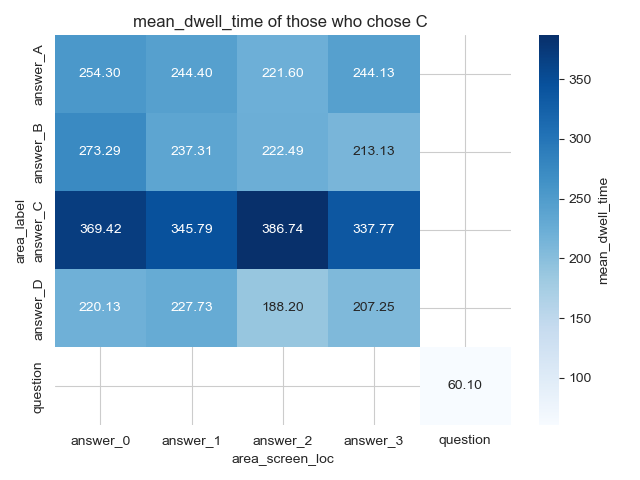
\includegraphics[width=\linewidth]{plots/matrix_plots/matrix_mean_dwell_time_C_gatherers.png}}
      \end{subcaptionbox}
      \hfill
      \begin{subcaptionbox}{Answered D\label{fig:D_dt_g}}[0.45\textwidth]
        {\centering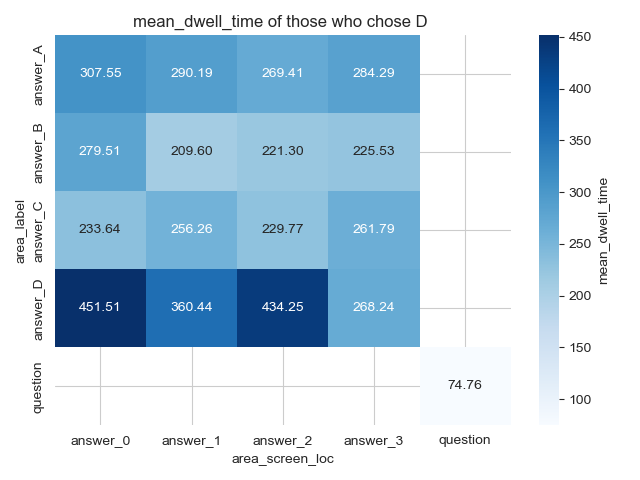
\includegraphics[width=\linewidth]{plots/matrix_plots/matrix_mean_dwell_time_D_gatherers.png}}
      \end{subcaptionbox}
      
      \caption{Mean Dwell Time by selected answer}
  \label{fig:fourimages4}
\end{figure}
\newpage

\subsection{First and Last visitations by labels / locations}

Last Time - no separation into ABCD, no last visits. 
\\

\textbf{First Visits}

\begin{figure}[H]
  \centering
  % First row of images
  \begin{subcaptionbox}{Area Label - A \label{fig:al_a}}[0.45\textwidth]
    {\centering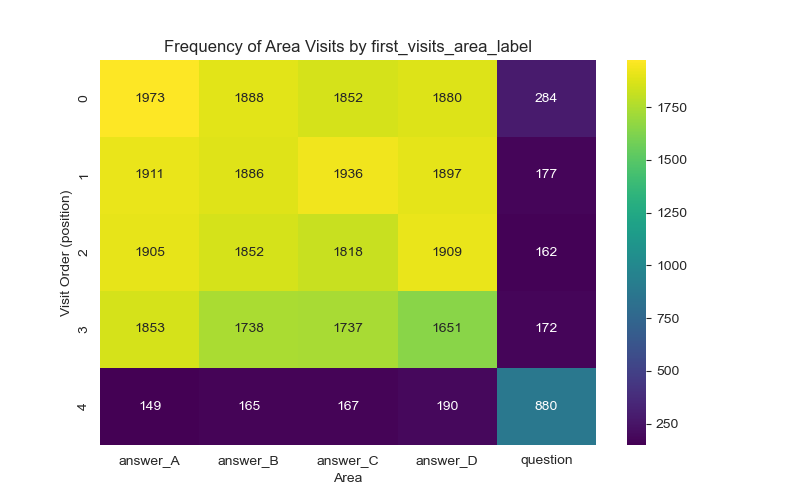
\includegraphics[width=\linewidth]{plots/visits/matrix__first_visits_area_label_hunters_A.png}}
  \end{subcaptionbox}
  \hfill
  \begin{subcaptionbox}{Area Label - B\label{fig:al_b}}[0.45\textwidth]
    {\centering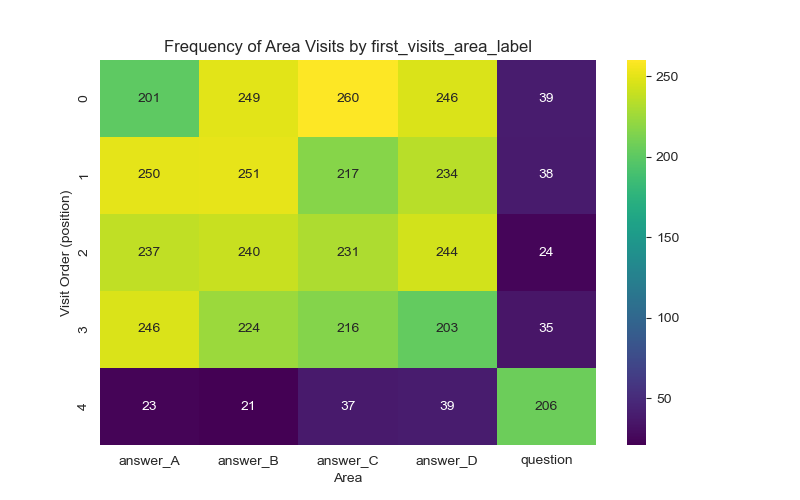
\includegraphics[width=\linewidth]{plots/visits/matrix__first_visits_area_label_hunters_B.png}}
  \end{subcaptionbox}
  
  \vspace{1em} % Vertical spacing between rows

  % Second row of images
  \begin{subcaptionbox}{Area Label - C\label{fig:al_c}}[0.45\textwidth]
    {\centering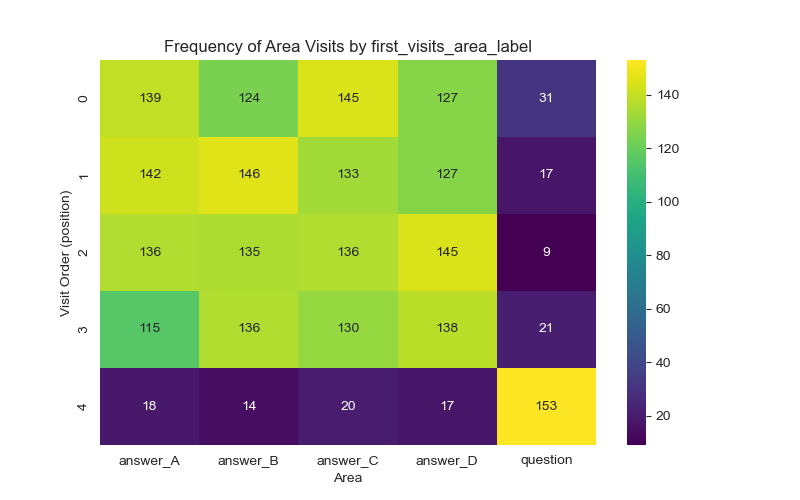
\includegraphics[width=\linewidth]{plots/visits/matrix__first_visits_area_label_hunters_C.png}}
  \end{subcaptionbox}
  \hfill
  \begin{subcaptionbox}{Area Label - D\label{fig:al_d}}[0.45\textwidth]
    {\centering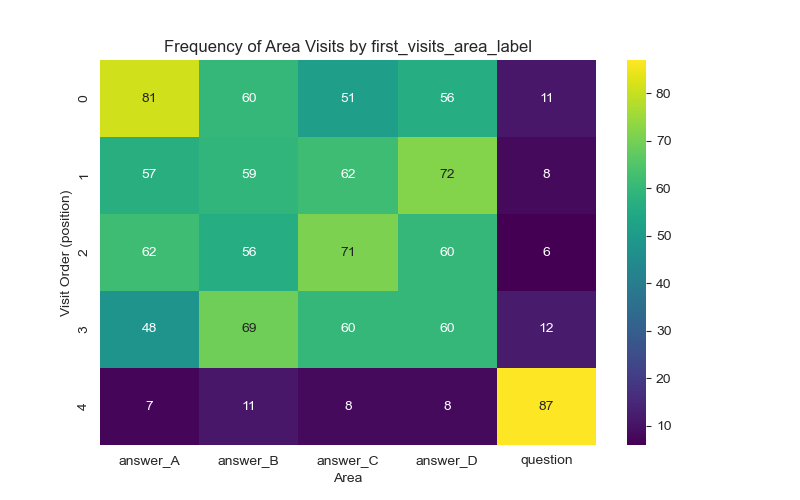
\includegraphics[width=\linewidth]{plots/visits/matrix__first_visits_area_label_hunters_D.png}}
  \end{subcaptionbox}
  
  \caption{First Visits}
  \label{fig:fourimages1}
\end{figure}



\begin{figure}[H]
  \centering
  % First row of images
  \begin{subcaptionbox}{Screen Location - A \label{fig:sl_a}}[0.45\textwidth]
    {\centering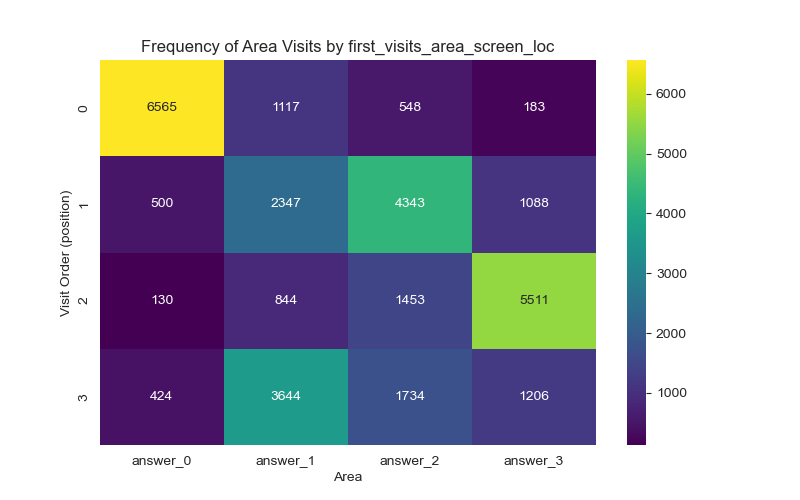
\includegraphics[width=\linewidth]{plots/visits/matrix__first_visits_area_screen_loc_hunters_A.png}}
  \end{subcaptionbox}
  \hfill
  \begin{subcaptionbox}{Screen Location - B\label{fig:sl_b}}[0.45\textwidth]
    {\centering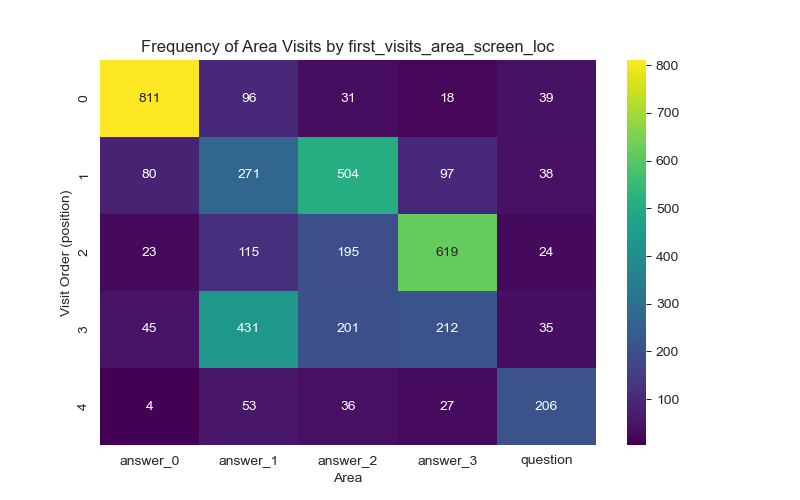
\includegraphics[width=\linewidth]{plots/visits/matrix__first_visits_area_screen_loc_hunters_B.png}}
  \end{subcaptionbox}
  
  \vspace{1em} % Vertical spacing between rows

  % Second row of images
  \begin{subcaptionbox}{Screen Location - C\label{fig:sl_c}}[0.45\textwidth]
    {\centering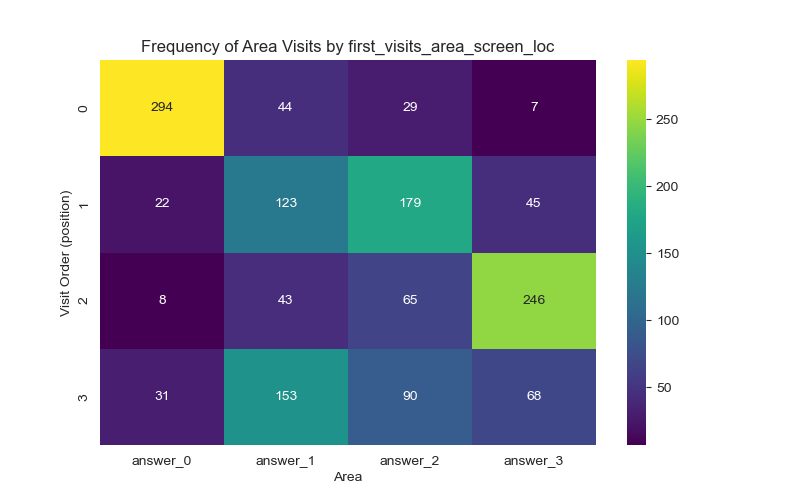
\includegraphics[width=\linewidth]{plots/visits/matrix__first_visits_area_screen_loc_hunters_C.png}}
  \end{subcaptionbox}
  \hfill
  \begin{subcaptionbox}{Screen Location - D\label{fig:sl_d}}[0.45\textwidth]
    {\centering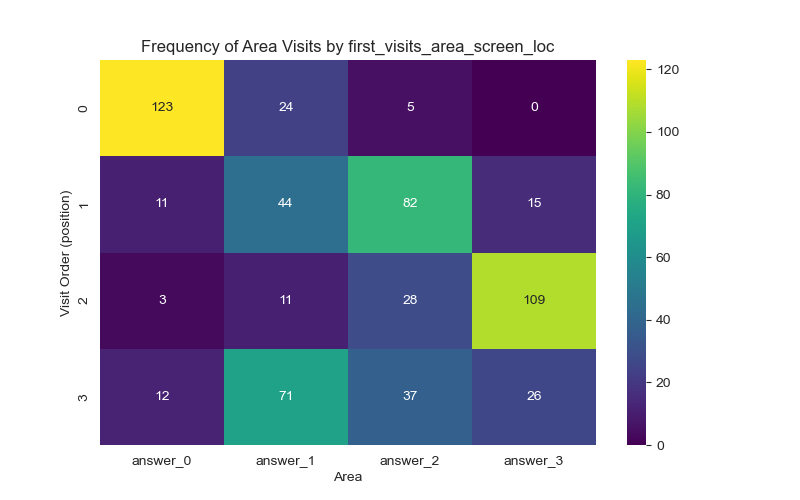
\includegraphics[width=\linewidth]{plots/visits/matrix__first_visits_area_screen_loc_hunters_D.png}}
  \end{subcaptionbox}
  
  \caption{First Visits}
  \label{fig:fourimages2}
\end{figure}



\newpage
\textbf{Last Visits}


\begin{figure}[H]
  \centering
  % First row of images
  \begin{subcaptionbox}{Area Label - A \label{fig:al_a}}[0.45\textwidth]
    {\centering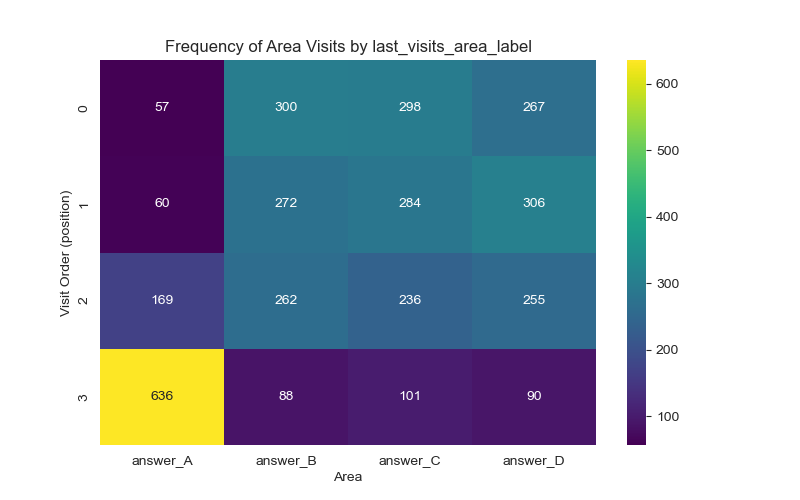
\includegraphics[width=\linewidth]{plots/visits/matrix__last_visits_area_label_gatherers_A.png}}
  \end{subcaptionbox}
  \hfill
  \begin{subcaptionbox}{Area Label - B\label{fig:al_b}}[0.45\textwidth]
    {\centering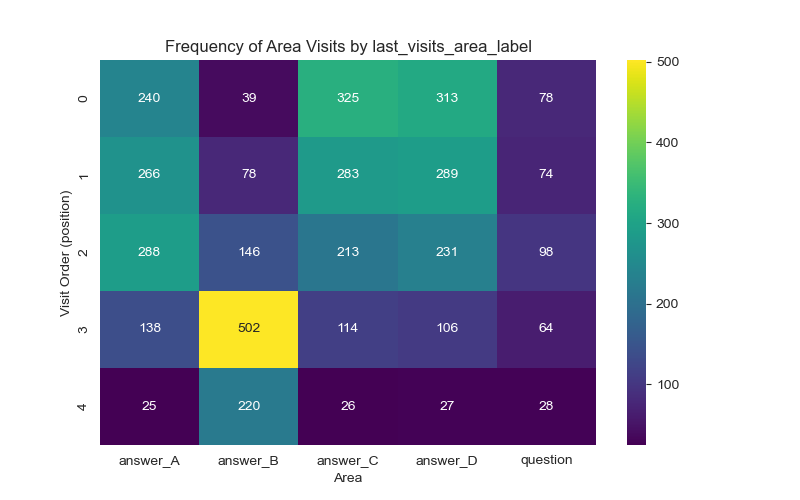
\includegraphics[width=\linewidth]{plots/visits/matrix__last_visits_area_label_gatherers_B.png}}
  \end{subcaptionbox}
  
  \vspace{1em} % Vertical spacing between rows

  % Second row of images
  \begin{subcaptionbox}{Area Label - C\label{fig:al_c}}[0.45\textwidth]
    {\centering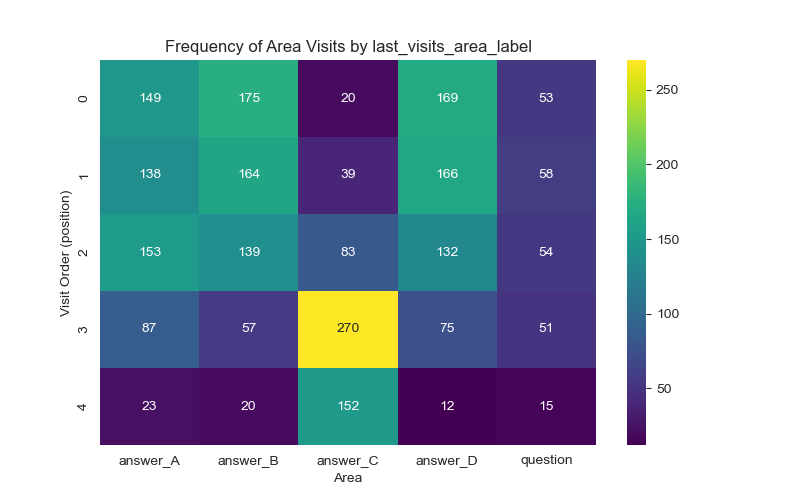
\includegraphics[width=\linewidth]{plots/visits/matrix__last_visits_area_label_gatherers_C.png}}
  \end{subcaptionbox}
  \hfill
  \begin{subcaptionbox}{Area Label - D\label{fig:al_d}}[0.45\textwidth]
    {\centering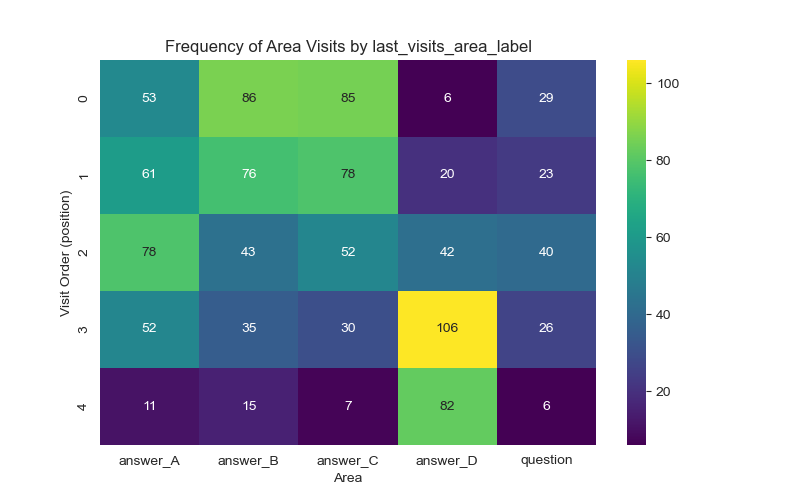
\includegraphics[width=\linewidth]{plots/visits/matrix__last_visits_area_label_gatherers_D.png}}
  \end{subcaptionbox}
  
  \caption{Last Visits}
  \label{fig:fourimages3}
\end{figure}




\begin{figure}[H]
  \centering
  % First row of images
  \begin{subcaptionbox}{Screen Location - A \label{fig:sl_a}}[0.45\textwidth]
    {\centering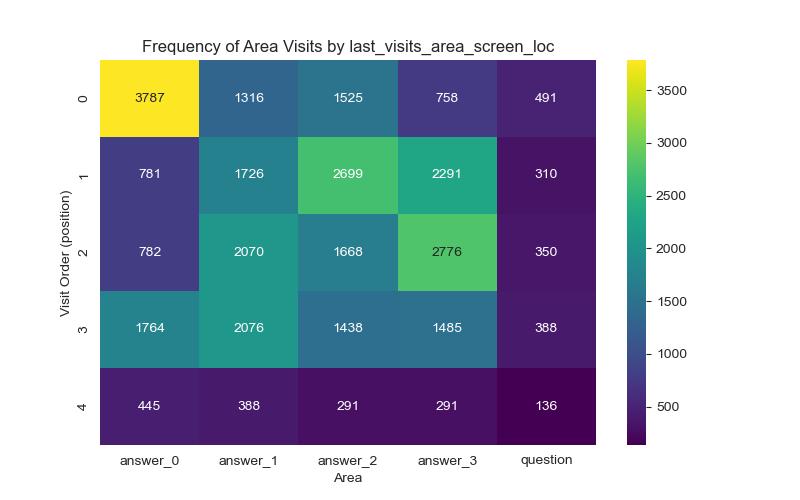
\includegraphics[width=\linewidth]{plots/visits/matrix__last_visits_area_screen_loc_gatherers_A.png}}
  \end{subcaptionbox}
  \hfill
  \begin{subcaptionbox}{Screen Location - B\label{fig:sl_b}}[0.45\textwidth]
    {\centering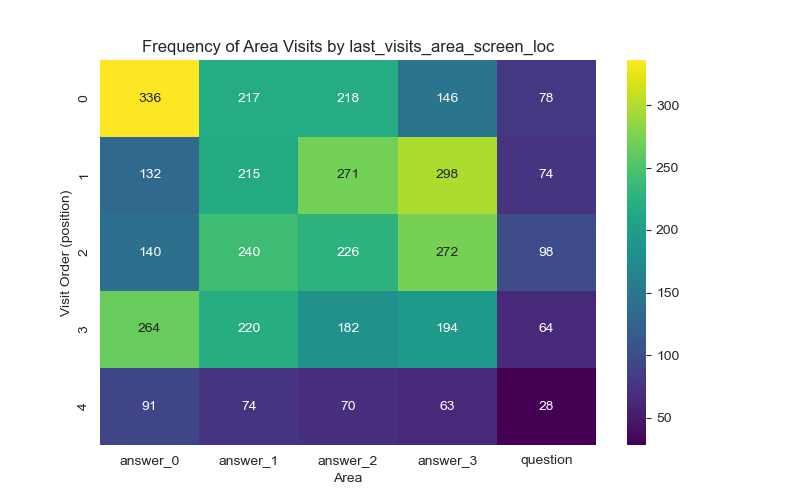
\includegraphics[width=\linewidth]{plots/visits/matrix__last_visits_area_screen_loc_gatherers_B.png}}
  \end{subcaptionbox}
  
  \vspace{0.5em} % Vertical spacing between rows

  % Second row of images
  \begin{subcaptionbox}{Screen Location - C\label{fig:sl_c}}[0.45\textwidth]
    {\centering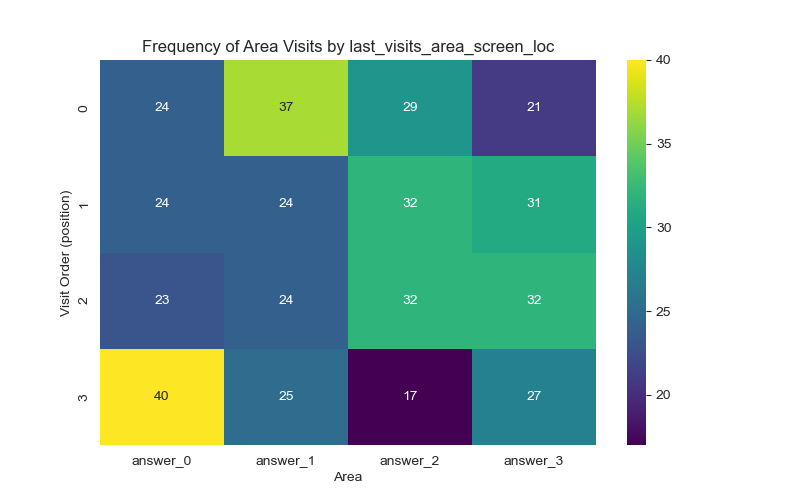
\includegraphics[width=\linewidth]{plots/visits/matrix__last_visits_area_screen_loc_gatherers_C.png}}
  \end{subcaptionbox}
  \hfill
  \begin{subcaptionbox}{Screen Location - D\label{fig:sl_d}}[0.45\textwidth]
    {\centering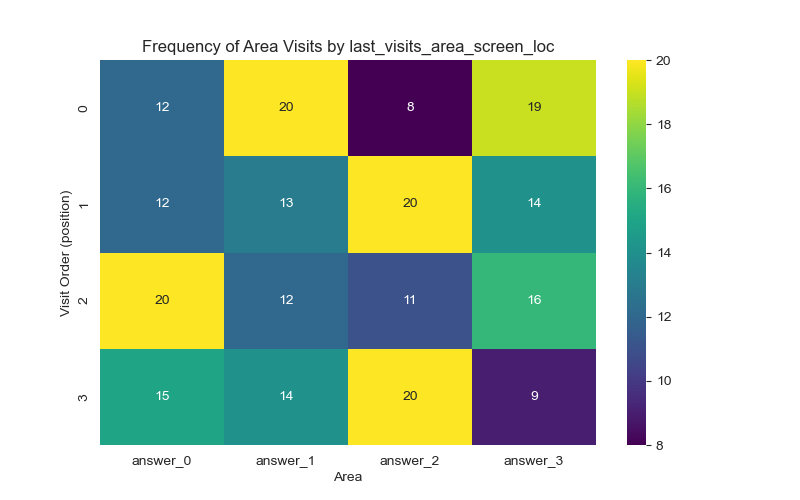
\includegraphics[width=\linewidth]{plots/visits/matrix__last_visits_area_screen_loc_gatherers_D.png}}
  \end{subcaptionbox}
  
  \caption{Last Visits}
  \label{fig:fourimages4}
\end{figure}


\begin{figure}[H]
    \centering
    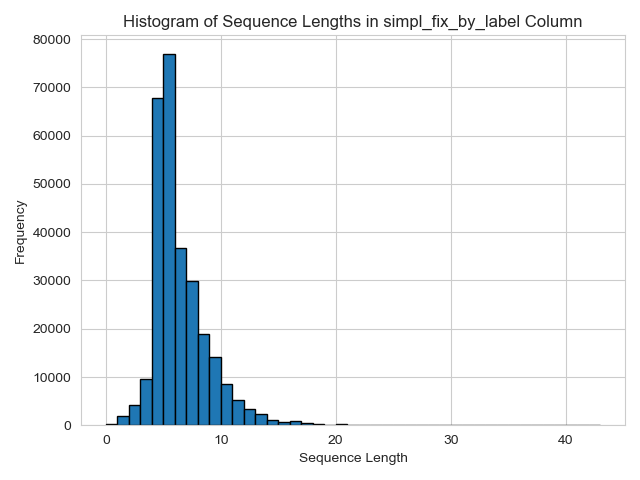
\includegraphics[width=1\linewidth]{plots/sequence_freq/simpl_fix_by_label.png}
    \caption{Simple Sequence Length}
    \label{fig:length}
\end{figure}
Clockwise pattern of last visits is spillover of short sequences 



\newpage
\section{Histograms of frequencies (first/last visits)}


\textbf{First Visits}
\begin{figure}[H]
    \centering
    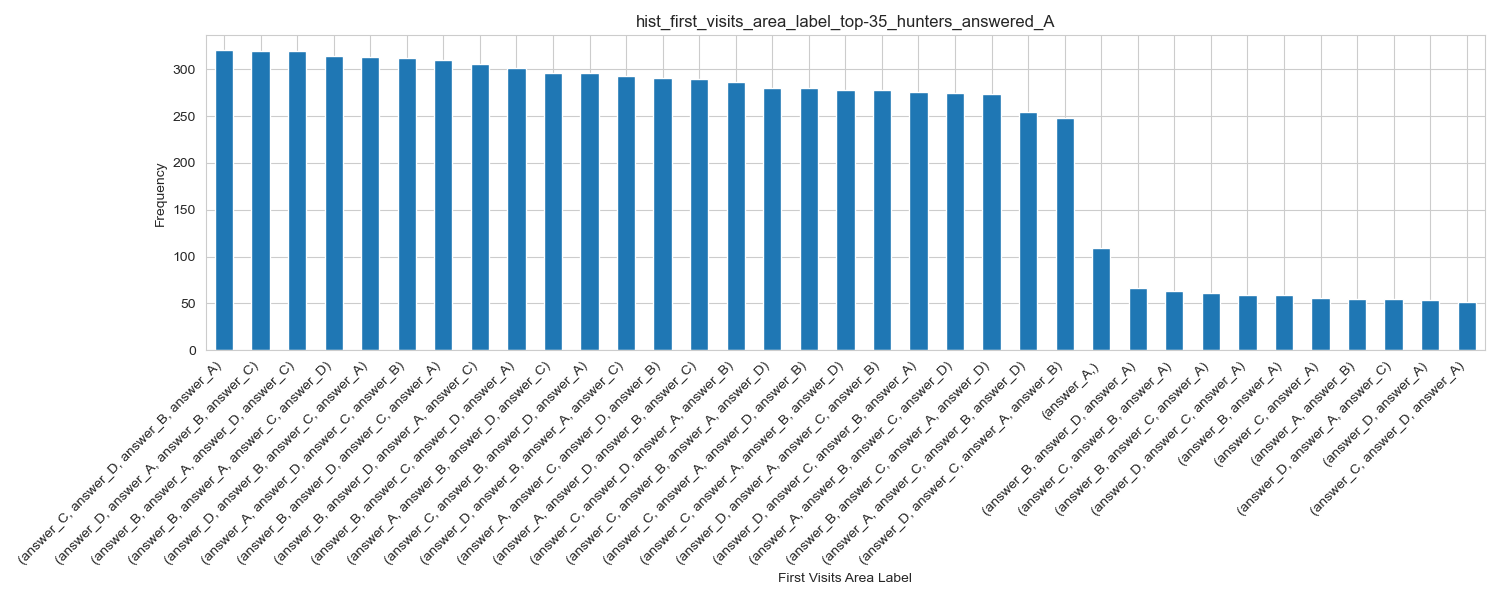
\includegraphics[width=1\linewidth]{plots/visits_hists/hist_first_visits_area_label_top-35_hunters_answered_A.png}
    \caption{First Visits by Label (answ - A)}
    \label{fig:sl_h}
\end{figure}




\begin{figure}[H]
    \centering
    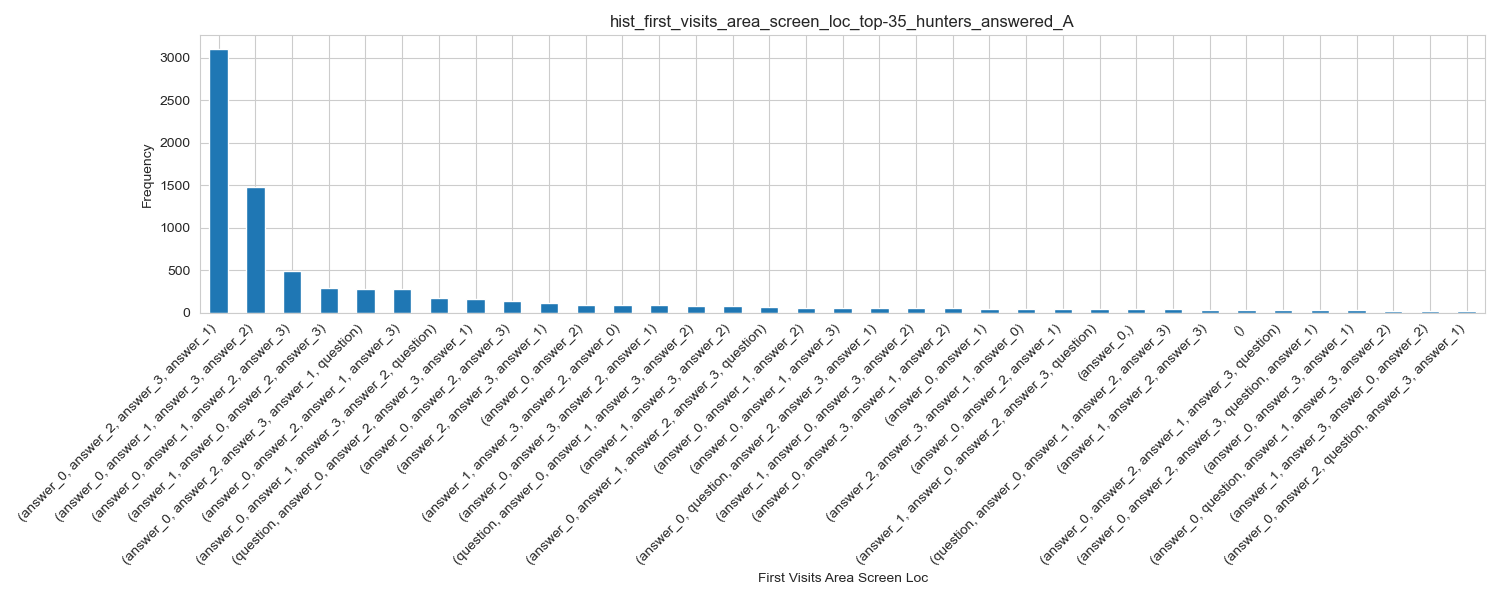
\includegraphics[width=1\linewidth]{plots/visits_hists/hist_first_visits_area_screen_loc_top-35_hunters_answered_A.png}
    \caption{First Visits by Location (answ - A)}
    \label{fig:sl_h}
\end{figure}


\newpage
\textbf{Last Visits}
\begin{figure}[H]
    \centering
    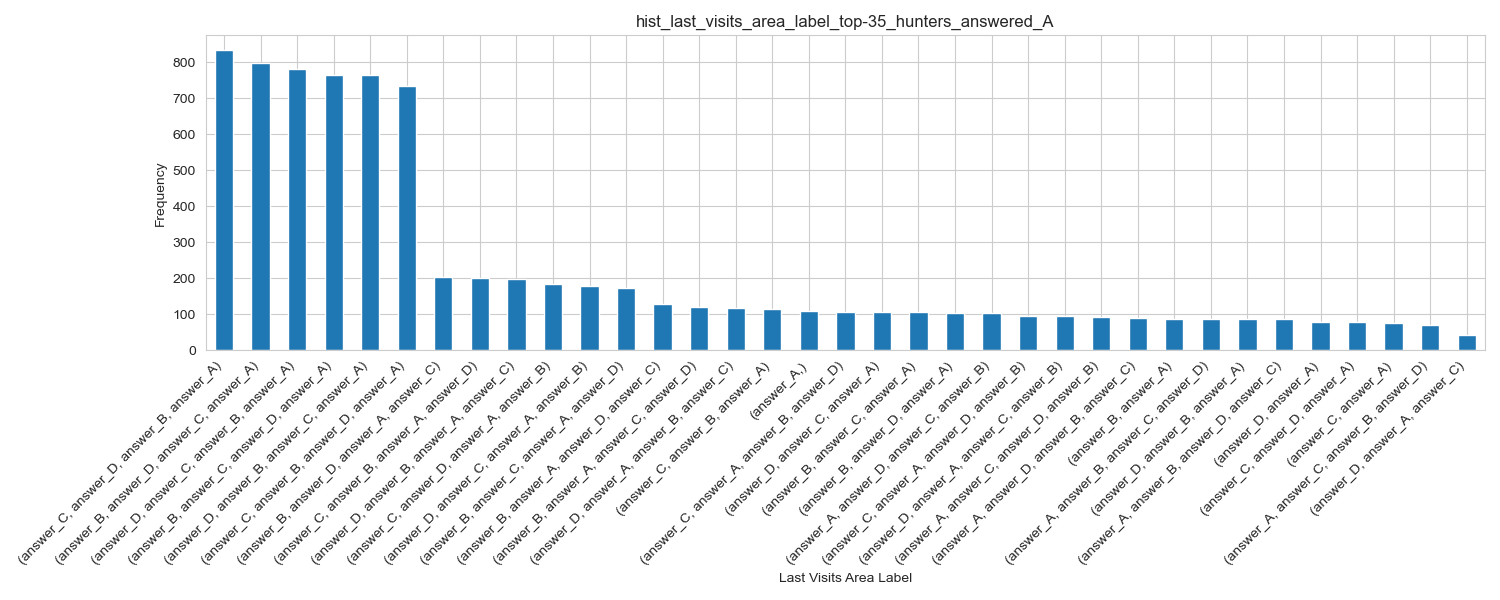
\includegraphics[width=1\linewidth]{plots/visits_hists/hist_last_visits_area_label_top-35_hunters_answered_A.png}
    \caption{Last Visits by Label (answ - A)}
    \label{fig:sl_h}
\end{figure}




\begin{figure}[H]
    \centering
    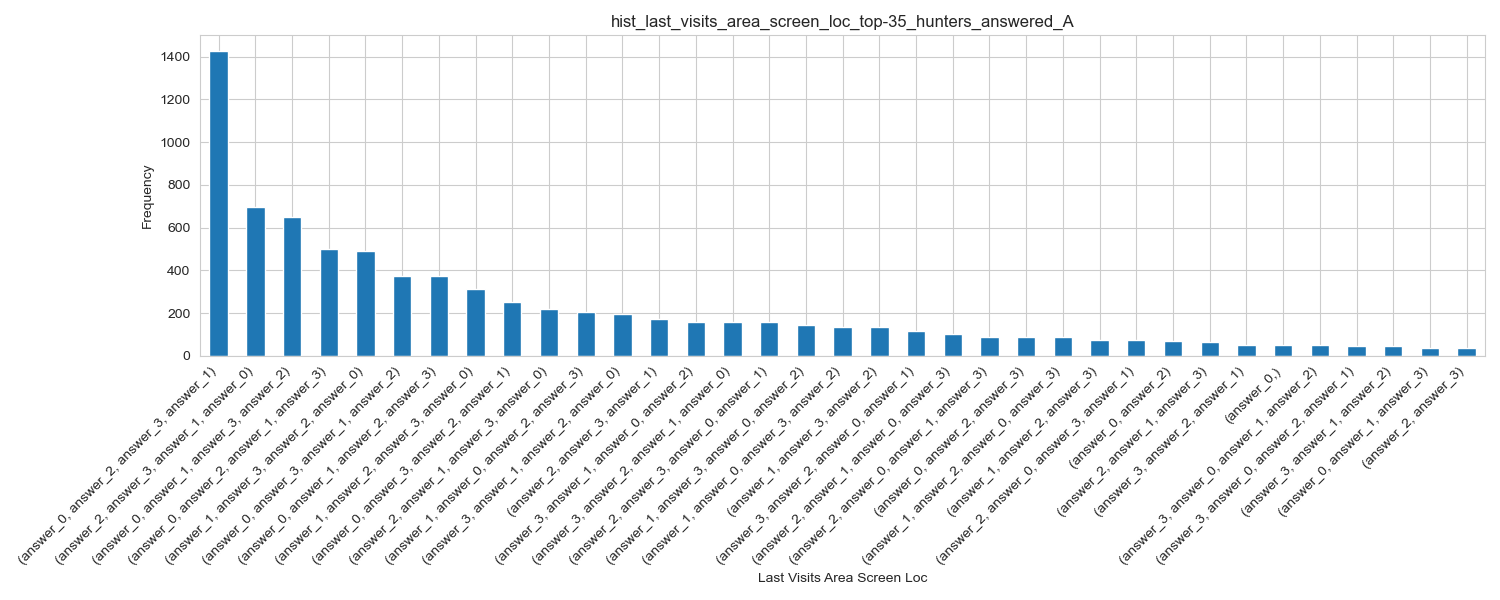
\includegraphics[width=1\linewidth]{plots/visits_hists/hist_last_visits_area_screen_loc_top-35_hunters_answered_A.png}
    \caption{Last Visits by Location (answ - A)}
    \label{fig:sl_h}
\end{figure}


\newpage
\section{Random participant (first) strategies}

\begin{figure}[H]
    \centering
    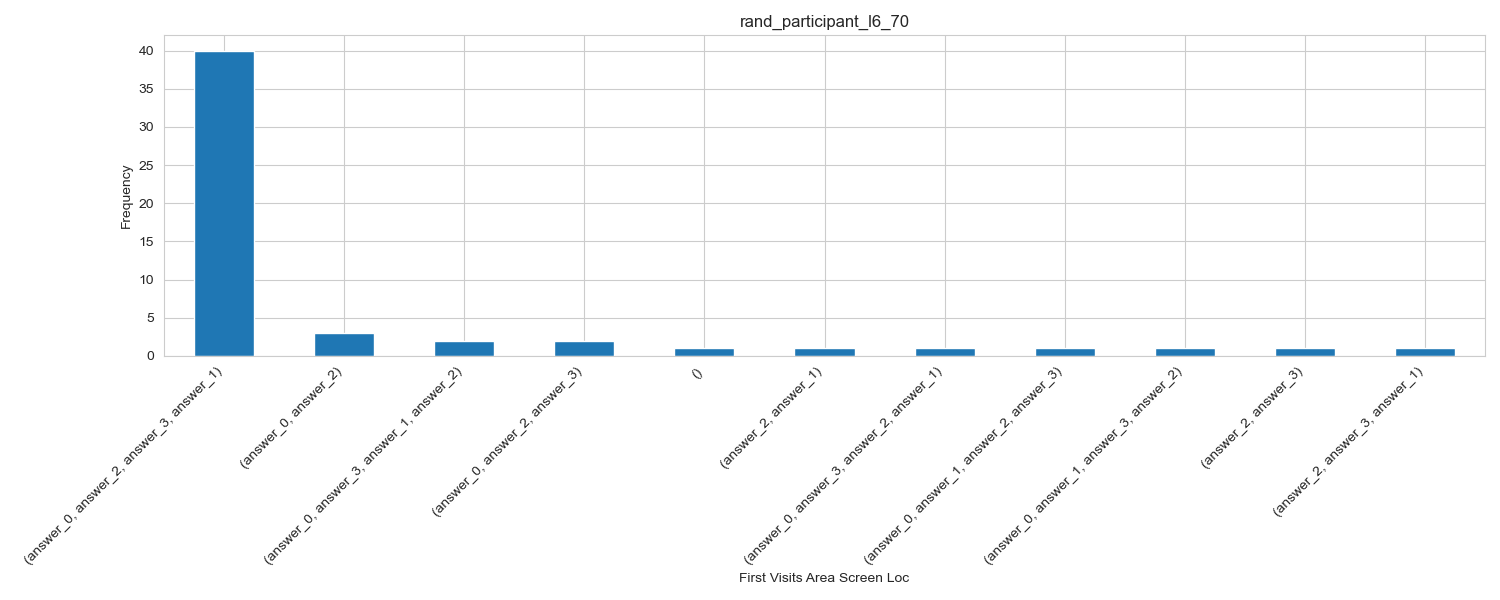
\includegraphics[width=1\linewidth]{plots/visits_hists/rand_participant_l6_70.png}
    \caption{Random Gatherer}
    \label{fig:sl_h}
\end{figure}
\begin{figure}[H]
    \centering
    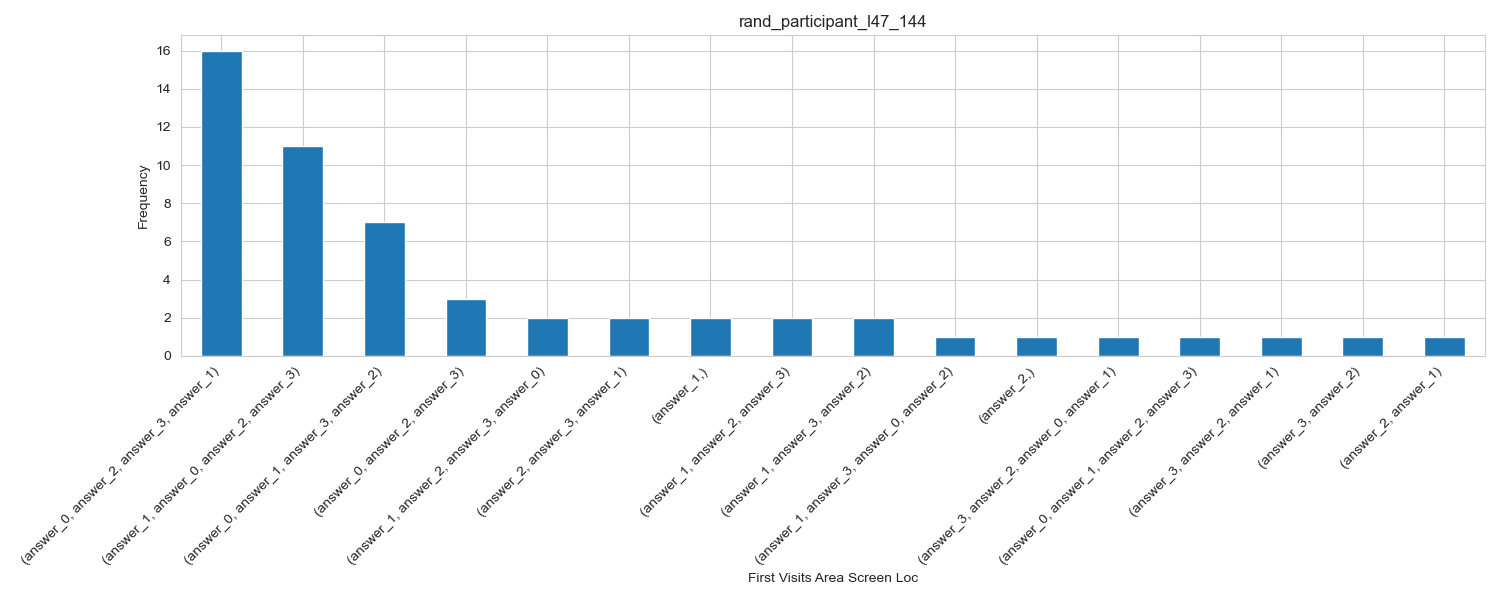
\includegraphics[width=1\linewidth]{{plots/visits_hists/rand_participant_l47_144}}
    \caption{Random Hunter}
    \label{fig:sl_h}
\end{figure}

Have the beginning and the end - what's in the middle?

\newpage
\section{Strategy dominance analysis}

Do people remain consistent in their approach?

\textbf{Hunters}

\begin{figure}[H]
    \centering
    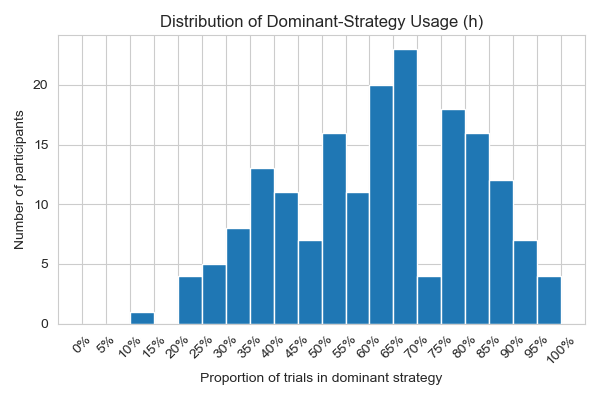
\includegraphics[width=0.70\linewidth]{{plots/strategies/dominant_prop_first_visits_area_screen_loc_h.png}}
    \label{fig:sl_h}
\end{figure}

\begin{figure}[H]
    \centering
    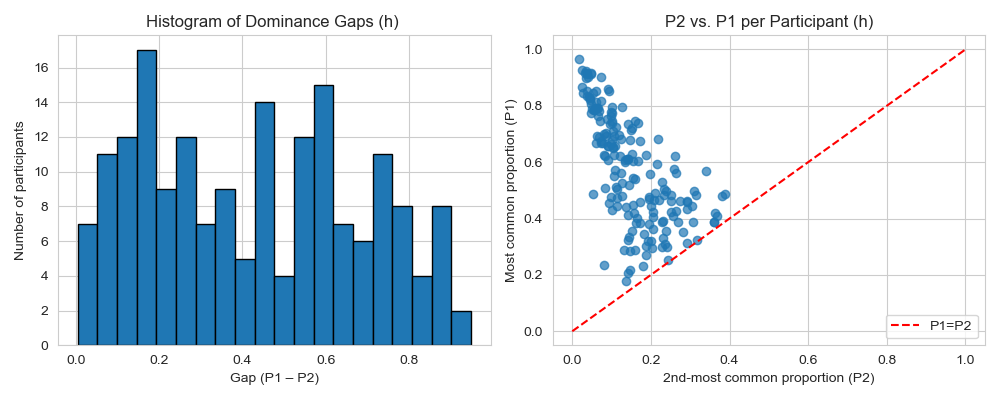
\includegraphics[width=0.9\linewidth]{{plots/strategies/dominance_gap_first_visits_area_screen_loc_h.png}}
    \label{fig:sl_h}
\end{figure}


\begin{figure}[H]
    \centering
    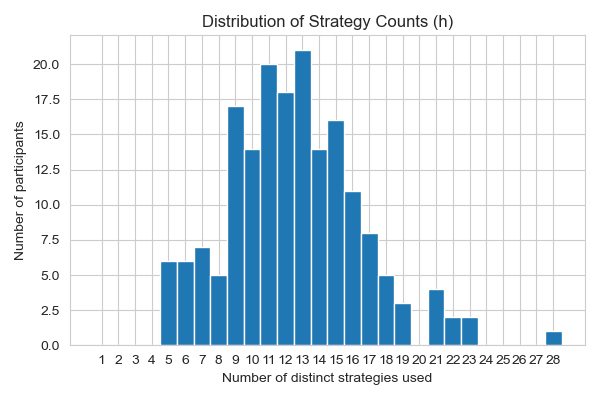
\includegraphics[width=0.70\linewidth]{{plots/strategies/dom_str_counts_first_visits_area_screen_loc_h.png}}
    \label{fig:sl_h}
\end{figure}

\newpage
\textbf{Gatherers}

\begin{figure}[H]
    \centering
    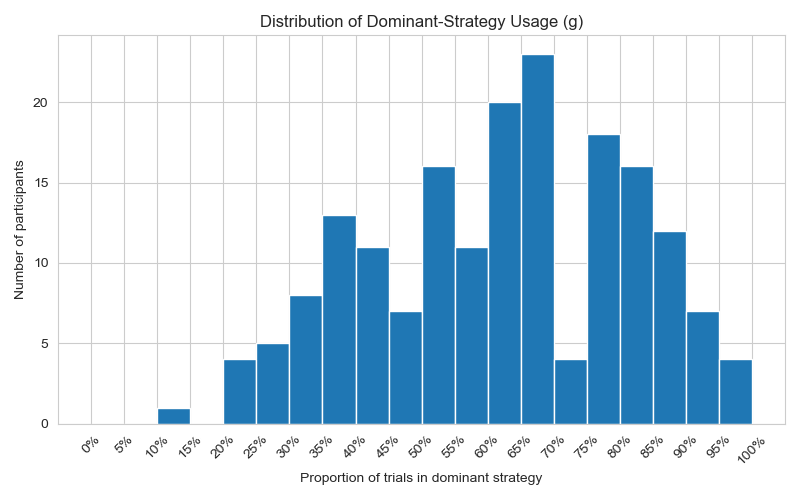
\includegraphics[width=0.70\linewidth]{{plots/strategies/dominant_prop_first_visits_area_screen_loc_g.png}}
    \label{fig:sl_h}
\end{figure}

\begin{figure}[H]
    \centering
    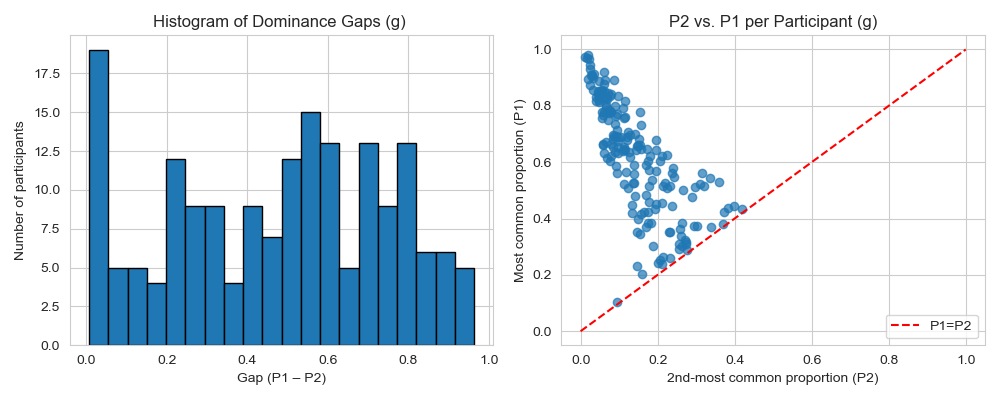
\includegraphics[width=0.9\linewidth]{{plots/strategies/dominance_gap_first_visits_area_screen_loc_g.png}}
    \label{fig:sl_h}
\end{figure}


\begin{figure}[H]
    \centering
    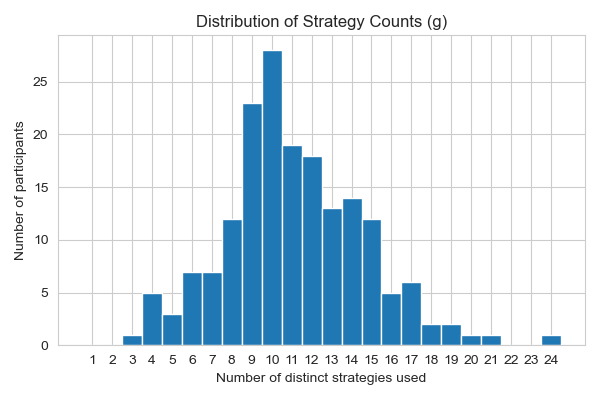
\includegraphics[width=0.70\linewidth]{{plots/strategies/dom_str_counts_first_visits_area_screen_loc_g.png}}
    \label{fig:sl_h}
\end{figure}

Is there a dominant strategy here that is not location based? (shortest text, etc)


\section{Distance Measure}

\begin{itemize}
    \item Levenshtein
    \item Scasim - works now, but needs to be seriously modified to use for this case
    \item 2D Levenshtein attempts: -mismatch, -euclidean.
    Each point is (location, label) pair - 


    \item Still need better way to integrate sequences
    
    
\end{itemize}


\section{Sequence Manipulations}

\begin{figure}[H]
    \centering
    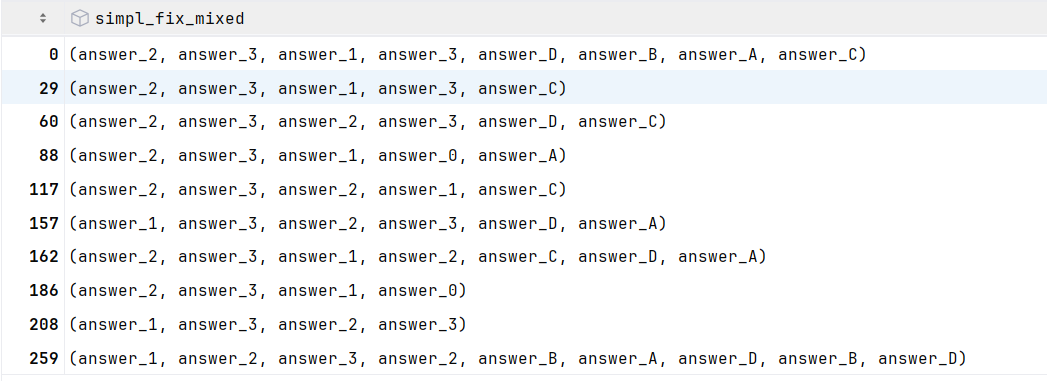
\includegraphics[width=1\linewidth]{plots/etc/dumb_mix.PNG}
    \caption{First 4 - loc, rest - label}
    \label{fig:enter-label}
\end{figure}


\begin{figure}[H]
    \centering
    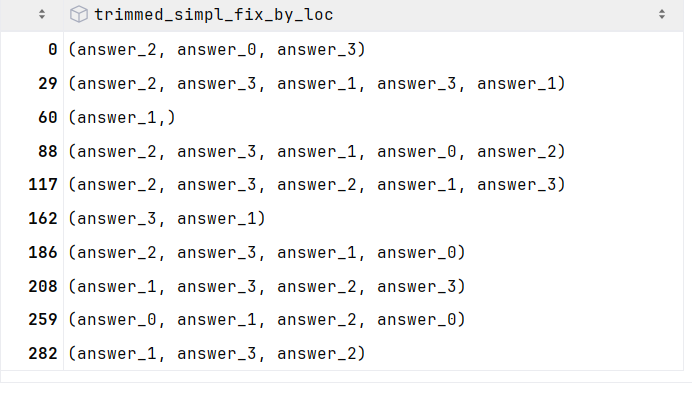
\includegraphics[width=1\linewidth]{plots/etc/trim_top_and_bottom.PNG}
    \caption{Trimmed Beginning and End}
    \label{fig:enter-label}
\end{figure}

\begin{figure}[H]
    \centering
    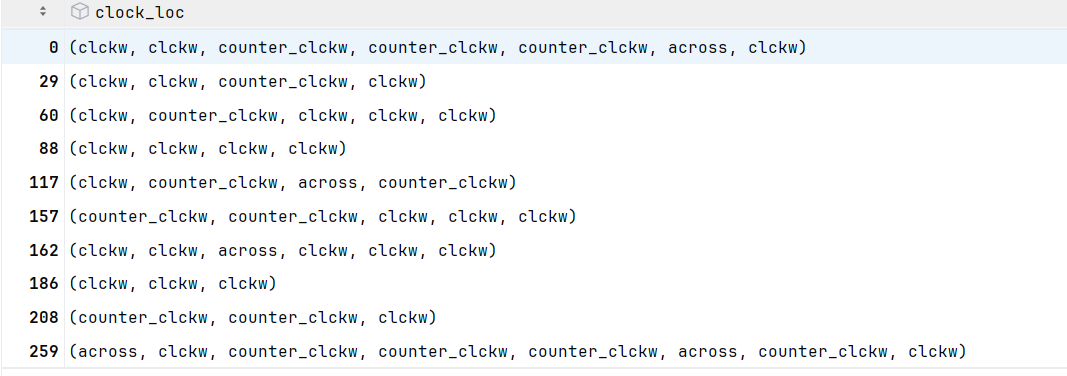
\includegraphics[width=1\linewidth]{plots/etc/clock.PNG}
    \caption{Transition Types}
    \label{fig:enter-label}
\end{figure}
Haven't done anything with this yet, but think it is promising

\section{Clustering}

Working on simplified (collapsed) sequences, otherwise unlikely to find any meaningful patterns across different texts.

\begin{itemize}
    \item KMEANS - over MDS fit space from distance matrix
    \item Agglomerative
    \item DBSAN
    \item HDBSAN - no need for n clusters!
\end{itemize}

Attempted some (small subset) hyperparameter tuning, though, no proper extensive runs have been made yet.

No results yet, though some sequence-distance-clustering combinations might have not been tested at all yet.

Not sure there are clusters at all in the space in which we look right now, might still need better representations. 

\end{document}